\documentclass[12pt]{article}
\topmargin        -0.5 in        % margins are relative to the default of 1 inch
\textheight      9.25 in
\oddsidemargin   0.0 in            % this is for pages 1, 3, 5, ...
\evensidemargin  0. in            % this is for pages 2, 3, 6, ...+++
\voffset		 0.0 in
\hoffset		 0.0 in
\textwidth       7.5 in
\headheight         0.0 in            % we don't have a running head nor
\headsep            0.0 in            % any extra space between head and text
\footskip			0.0 in
\parindent          0 pt
\usepackage[latin1]{inputenc}
\usepackage[english]{babel}
\usepackage{graphics,amssymb,amsmath,latexsym,graphicx,amsthm,mdwlist,multicol,multirow, enumerate,extsizes,setspace}
\usepackage[margin=.5in]{geometry}
%\usepackage{fancyhdr}
\usepackage[usenames]{color}
\newtheorem{thm}{Theorem}
\newtheorem{lemma}{Lemma}
\newtheorem{dfn}{Definition}
\newtheorem{ex}{Example}
\newtheorem{cor}{Corollary}
\newcommand{\DS}{\displaystyle}
\newcommand{\tbf}{\textbf}
%\pagestyle{fancy}   

\begin{document}

\begin{center}
 \large{\underline{Sec 7.1: Eigenvalues and Eigenvectors}}
\end{center}

\underline{HW}:\\ 

\vspace{.1in}


\underline{Question}: If A is an n x n matrix, do there exist nonzero vectors \tbf{x} in $R^n$ such that A\tbf{x} is a scalar multiple of \tbf{x}?

\begin{center}
$A\tbf{x} = \lambda \tbf{x}$
\end{center}


\underline{Vocab}:
\begin{itemize}
\item
The scalar ($\lambda$) is known as an \tbf{eigenvalue} of the matrix A.

\item
The (nonzero) vector \tbf{x} is called an \tbf{eigenvector} of A corresponding to $\lambda$

\item
The terms eigenvalue and eigenvector are derived from the German word \textit{Eigenwert} meaning ``proper value."
\end{itemize}

\vspace{.1in}

\underline{Geometrically}:

\begin{center}
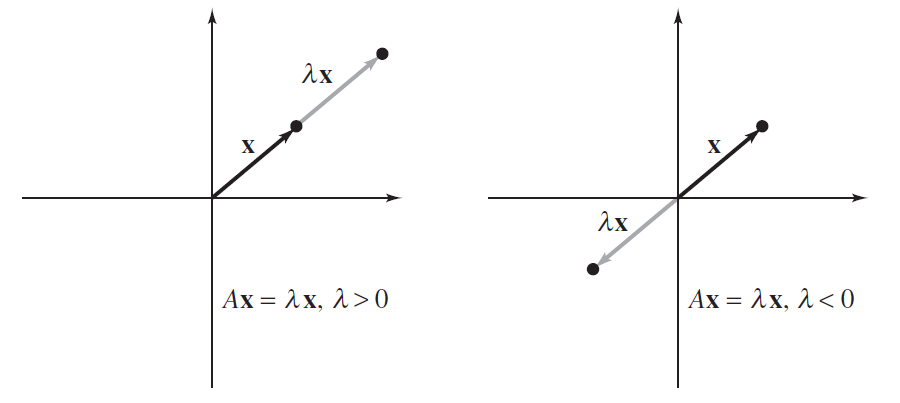
\includegraphics[width=5in]{ex1}
\end{center}

\begin{ex}

For the matrix $A = \begin{bmatrix}
2	&	0	\\
0	&	-1	\\
\end{bmatrix}$ verify that $\tbf{x} = (1,0)$ is an eigenvector of A corresponding to the eigenvalue $\lambda = 2$.
\end{ex}







\pagebreak
%%%%%%%%%%%%%%%%%%%%%%%%%%%%%%%%%%%%%%%%%%%%%%%%%%%%%%%%%%%%%%%%%%%%%
\begin{center}
\underline{Finding Eigenvalues and Eigenvectors}
\end{center}

\begin{ex}
Write $A\tbf{x} = \lambda \tbf{x}$ as a homogeneous system.
\end{ex}
\vfill

\underline{Note}: The homogeneous system of equations has \tbf{nonzero} solutions if and only if the coefficient matrix $(\lambda I - A)$ is \tbf{not} invertible. That is,  if and only if the determinant of $(\lambda I - A)$ is zero.


\vspace{.1in}

\begin{thm} Eigenvalues and Eigenvectors of a Square Matrix

Let A be an n x n matrix.

\begin{enumerate}
\item
\underline{Eigenvalues}: An eigenvalue of A is a scalar $\lambda$ such that 
\begin{center}
$det(\lambda I - A) = 0$
\end{center}


\item
\underline{Eigenvectors}: The eigenvectors of A corresponding to $\lambda$ are the \tbf{nonzero} solutions of  
\begin{center}
$(\lambda I - A)\tbf{x} = \tbf{0}$
\end{center}

\end{enumerate}

\end{thm}

\vspace{.1in}

\begin{dfn} Characteristic Equation

The equation $det(\lambda I - A) = 0$ is called the \tbf{characteristic equation} of A. The eigenvalues of an n x n matrix correspond to the roots of the characteristic polynomial. The characteristic equation is a polynomial of degree n in the variable $\lambda$. (We will only consider the real roots of the equation and therefore only the real eigenvalues.)

\begin{center}
$\lvert (\lambda I - A) \rvert = \lambda^n + c_{n-1}\lambda^{n-1} + \ldots c_1\lambda + c_0$
\end{center}

\end{dfn}
\pagebreak
%%%%%%%%%%%%%%%%%%%%%%%%%%%%%%%%%%%%%%%%%%%%%%%%%%%%%%%%%%%%%%%%%%%%%%%55
\begin{thm} Eigenvectors of $\lambda$ form a Subspace


If A is an n x n matrix with an eigenvalues $\lambda$, then the \tbf{set} of all eigenvectors of $\lambda$ together with the zero vector is a subspace of $R^n$. This subspace is called the \tbf{eigenspace} of $\lambda$.

\begin{center}
$\{ \tbf{0 } \} \cup \{ \tbf{x } \lvert \tbf{ x}$ is an eigenvector of $\lambda\}$
\end{center}



\end{thm}




\pagebreak
%%%%%%%%%%%%%%%%%%%%%%%%%%%%%%%%%%%%%%%%%%%%%%%%%%%%%%%%%%%%%%%%%%%%
\begin{ex} 

Find the eigenvalues and corresponding eigenvectors of A.

\begin{center}
$A = \begin{bmatrix}
2	&	-12	\\
1	&	-5	\\
\end{bmatrix}$
\end{center}

\end{ex}

\begin{enumerate}[a)]
\item
\underline{Characteristic Polynomial}:

\vfill

\item
\underline{Eigenvalues}:

\vfill

\item
\underline{Eigenvectors}:

\vfill


\item
\underline{Eigenspace}:
\vfill

\end{enumerate}

\pagebreak
%%%%%%%%%%%%%%%%%%%%%%%%%%%%%%%%%%%%%%%%%%%%%%%%%%%%%%%%%%%%%%%%%%%
\begin{thm} Eigenvalues of a Triangular Matrix

If A is an n x n matrix, then its eigenvalues are the entries on its main diagonal. 
\end{thm}

\underline{Note}: The proof follows from the fact that the determinant of a triangular matrix is the product of its diagonal elements. (If necessary, recall the rules of determinants from Chapter 3.)

\vspace{.1in}

\begin{ex}

Find the eigenvalues for the following matrix.

\begin{center}
$A = \begin{bmatrix}
2	&	0	&	0\\
-1	&	1	&	0\\
5	&	3	&	-3\\
\end{bmatrix}$
\end{center}
\end{ex}

\vfill

\begin{dfn} Diagonal Matrix

A matrix that is both upper and lower triangular is called a \tbf{diagonal} matrix.

\end{dfn}

\vfill




\begin{center}
\underline{Eigenvalues and Eigenvectors of Linear Transformations}
\end{center}

Eigenvectors and eigenvalues can also be defined in terms of linear transformations. 

\begin{dfn}
Let V be a \tbf{finite} dimensional vector space and let  $T: V \rightarrow V$  be a linear transformation. Then $\lambda$ is an eigenvalue for T if there exists a non-zero vector \tbf{x} in V such that

\begin{center}
$T(\tbf{x}) = \lambda \tbf{x}$  
\end{center}

\end{dfn}

\vspace{.1in}


Let $ T: R^3 \rightarrow R^3$ whose matrix relative to the standard basis is:

\begin{center}
$A = \begin{bmatrix}
1	&	3	&	0	\\
3	&	1	&	0	\\
0	&	0	&	-2	\\
\end{bmatrix}$
\end{center}

Then the matrix of T relative to the nonstandard basis $B'$ is a diagonal matrix. (From Sec 6.4)

\begin{multicols}{2}

$A' = \begin{bmatrix}
4	&	0	&	0\\
0	&	-2	&	0\\
0	&	0	&	-2\\
\end{bmatrix}$


$B' = \{ (1, 1, 0), (1, -1, 0), (0, 0, 1) \}$

\end{multicols}

\vspace{.1in}

\underline{Goal}: For a given transformation T, find a basis $B'$ whose corresponding matrix is diagonal.


\pagebreak
%%%%%%%%%%%%%%%%%%%%%%%%%%%%%%%%%%%%%%%%%%%%%%%%%%%%%%%%%%%%%%%%%%%%%%%%%%%

\begin{ex}

Find eigenvalues and corresponding eigenspace of 

\begin{center}

$A = \begin{bmatrix}
1	&	3	&	0\\
3	&	1	&	0\\
0	&	0	&	-2\\
\end{bmatrix}$

\end{center}
\end{ex}

\begin{enumerate}[a)]

\item
\underline{Characteristic Equation}:
\vfill

\item
\underline{Eigenvalues}:
\vfill

\item
\underline{Basis for Eigenspaces}:
\vfill
\end{enumerate}

\pagebreak
%%%%%%%%%%%%%%%%%%%%%%%%%%%%%%%%%%%%%%%%%%%%%%%%%%%%%%%%%%%%%%%%%%%%%%%%%%
\begin{center}
\underline{Surprising Results from Previous Example}
\end{center}

\begin{itemize}
\item
Let $T: R^3 \rightarrow R^3$ be the standard matrix whose matrix is A.

\item
Let $B'$ be the basis of $R^3$ made up of the three linearly independent eigenvectors.

\item
Then the transition matrix of T relative to $B'$ is diagonal. 

\item
The eigenvalues of A are the main diagonal entries of the matrix $A'$.


\end{itemize}


\vspace{.1in}

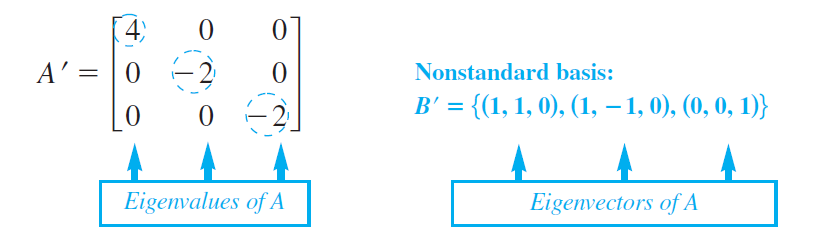
\includegraphics[width=5in]{ex2}

















\end{document}